\documentclass[12pt,a4paper]{article} %(nie wiem kiedy) usunąłem tą linię i nie wiem czy tak było
%przykladowe pakiety
\usepackage[utf8]{inputenc}
\usepackage{polski}
\usepackage{graphicx}
\usepackage{caption}
\usepackage{amsmath} % w zasadzie tez mozna wywalic 
\usepackage{booktabs}
\usepackage{listings}
\usepackage{color}
\usepackage{geometry} 
\usepackage{biblatex}
\addbibresource{references.bib}

\geometry{
	a4paper,
	left = 2.5cm,
	right = 2.5cm,
	top = 2cm,
	bottom = 2cm
}

\begin{document}

\begin{titlepage}

\newcommand{\HRule}{\rule{\linewidth}{0.5mm}}

\center
 
\textsc{\LARGE Politechnika Wrocławska}\\[1.5cm] 
\textsc{\Large Zastosowanie informatyki w gospodarce}\\[0.5cm]

\HRule \\[0.5cm]
{ \huge \bfseries Relacje pomiędzy bytami w tekstach literackich - dokumentacja}\\[0.2cm]
\HRule \\[1.6cm]
 
 
\begin{minipage}{0.4\textwidth}
\begin{flushleft} \large
\emph{Lider grupy:}\\
Przemysław \textsc{Wujek} 234983\\
\emph{Skład grupy:}\\
Paweł \textsc{Czarnecki} 234974\\
Łukasz \textsc{Łupicki} 257536\\
Dawid \textsc{Piechota} 235851\\
Bartosz \textsc{Rodziewicz} 226105\\
Wojciech \textsc{Wójcik} 235621\\
\end{flushleft}
\end{minipage}
~
\begin{minipage}{0.4\textwidth}
\begin{flushright} \large
\emph{Prowadzący:} \\
dr inż. Tomasz \textsc{Walkowiak} 
\end{flushright}
\end{minipage}\\[4cm]

\vfill
{\large 4 kwietnia 2020}

\end{titlepage}
   
\newpage

\section{Prezentacja danych}

\subsection{Metoda prezentacji danych}
Do prezentacji wygenerowanych relacji został wybrany graf skierowany siłą (ang. \textit{force-directed graph}).
Algorytm rysowania takiego grafu wykorzystuje jedynie informacje zawarte w strukturze danych (węzły oraz połączenia między nimi).
Grafy wygenerowane za pomocą takich algorytmów są estetyczne i uporządkowane. Posiadają także niewielką ilość przecinających się połączeń \cite{yeet}. Te cechy są szczególnie przydatne w przypadku wizualizowania dużych zbiorów danych. Generowanie grafu polega na przypisaniu sił między zbiorem krawędzi i zbiorem węzłów w oparciu o ich względne pozycje, a następnie użyciu tych sił do symulacji ruchu krawędzi i węzłów lub do zminimalizowania ich energii\cite{yworks}. W pierwszym przypadku siły są liczone w czasie rzeczywistym, czego wynikiem jest graf, w którego układ może ingerować użytkownik (np. poprzez przeciąganie węzłów w inne pozycje). W drugim przypadku wyświetlenie grafu następuje po zminimalizowaniu sił, czego wynikiem jest statyczny graf. Odświeżanie widoku grafu w czasie rzeczywistym znacząco zwiększa czas minimalizacji sił, ponieważ widok grafu jest często odświeżany. Graf statyczny osiąga minimalne siły w dużo krótszym czasie, jednak pozbawiony jest możliwości interakcji z węzłami.\\

W celu przetestowania różnych metod prezentacji relacji, został utworzony projekt oparty na frameworku Vue. Użytkownik posiada możliwość wygenerowania grafu podając link do pliku z danymi [rys~\ref{fig:graph}]. Do generowania grafu została wykorzystana biblioteka D3.js \cite{d3}. Wybór biblioteki jest umotywowany wysoko konfigurowalną implementacją grafu skierowanego siłą.

\begin{figure}[h]
\caption{Wygenerowany graf współwystępowania postaci w Les Mis\'erables}
\frame{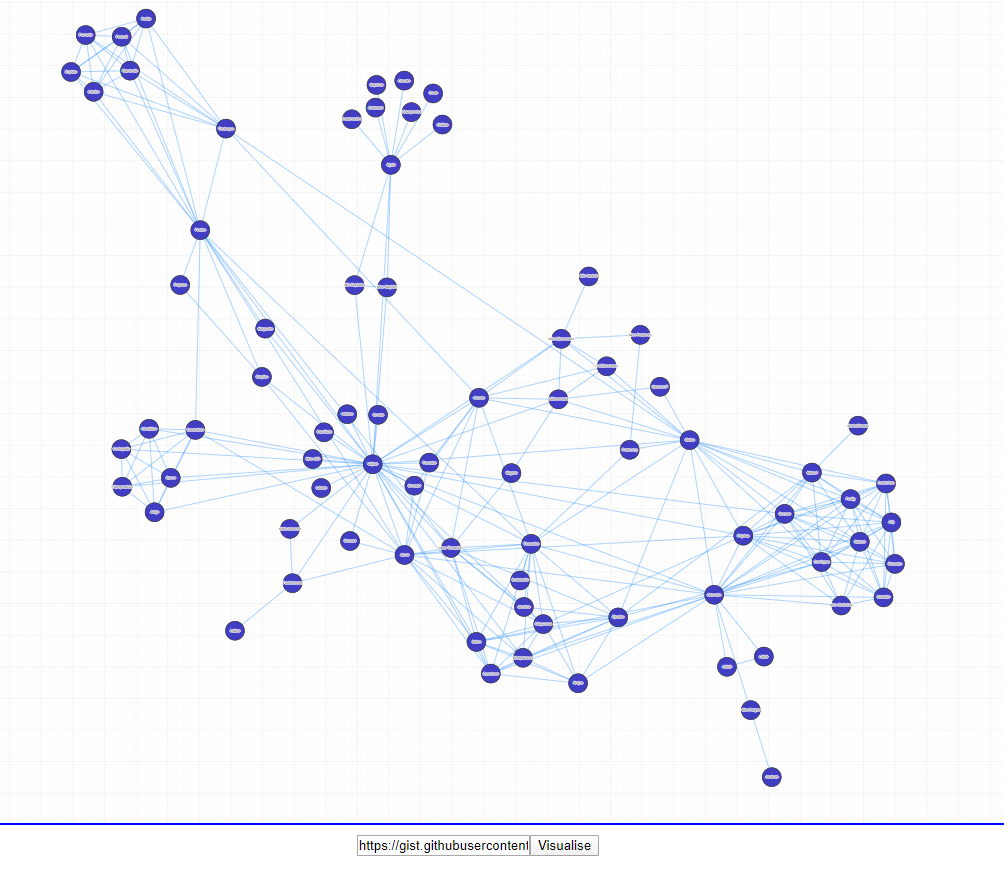
\includegraphics[width=13cm]{rys/fdGraph.png}}
\label{fig:graph}
\centering
\end{figure}

\subsection{Metoda prezentacji siły powiązań}

Wizualizację siły powiązań bytów można zrealizować na różne sposoby (Przykład na Rysunku \ref{fig:caw}). Od siły połączenia może zależeć między innymi:

\begin{itemize}
    \item kolor połączenia
    \item szerokość połączenia
    \item przezroczystość połączenia
    \item kształt połączenia (linia przerywana/ciągła etc.)
\end{itemize}

\begin{figure}[h]
\caption{Wizualizacja ze zmienną szerokością i kolorem połączenia}
\frame{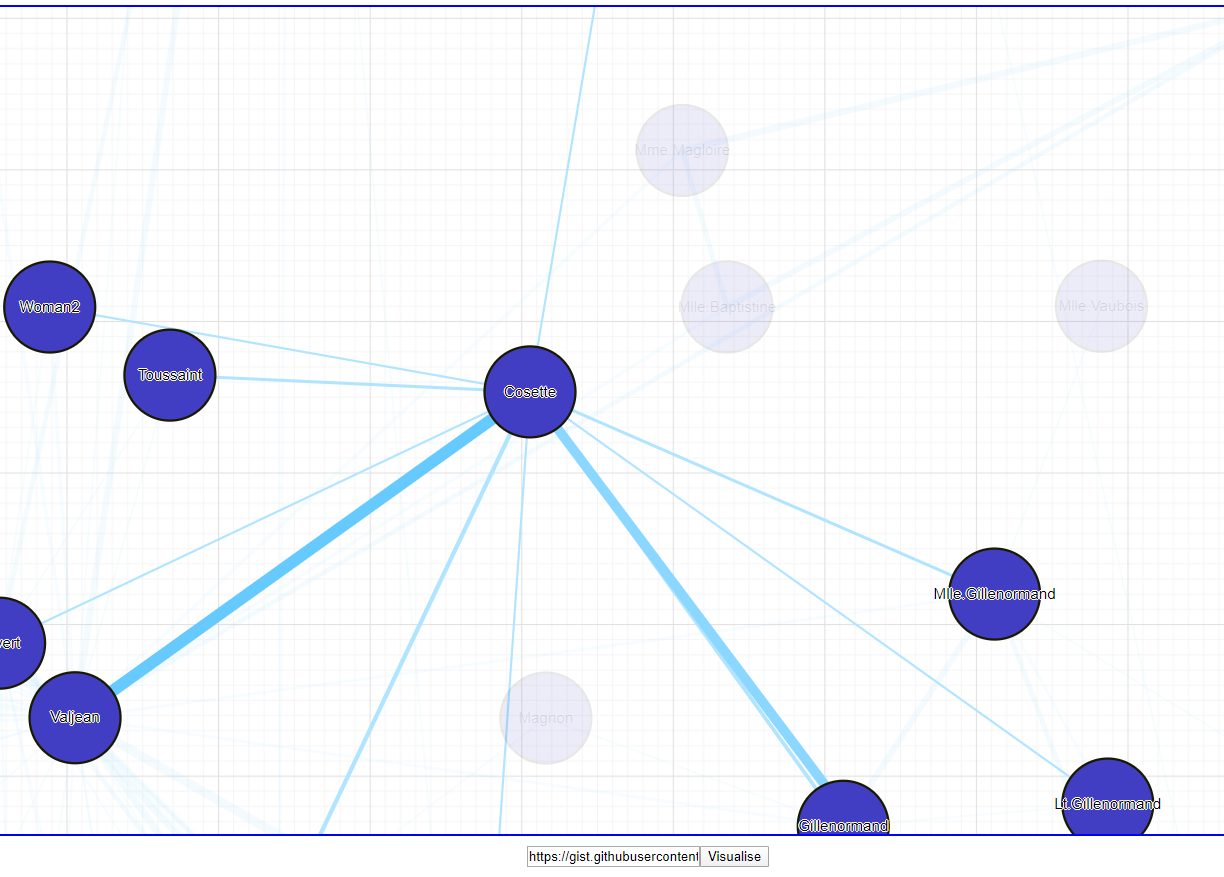
\includegraphics[width=13cm]{rys/caw2.png}}
\label{fig:caw}
\centering
\end{figure}

Jak do tej pory, wszystkie testy zostały przeprowadzone na jednym zbiorze danych (z noweli Les Mis\'erables). Po zaimplementowaniu narzędzia, które generuje zbiór danych na podstawie podanego tekstu, będzie można kontynuować testy i przeprowadzić analizę czytelności wybranych metod wizualizacji.

\newpage

\subsection{Dostępne akcje w reprezentacji graficznej}
W celu zapewnienia większej czytelności zostały zaimplementowane następujące funkcjonalności:
\begin{itemize}
    \item przybliżanie oraz oddalanie widoku kółkiem myszy [rys~\ref{fig:zoom}]
    \item zaznaczanie połączonych węzłów po najechaniu myszką [rys~\ref{fig:highlight}]
    \item przeciąganie węzłów
\end{itemize}


\begin{figure}[h]
\caption{Przybliżenie na grupę bytów}
\frame{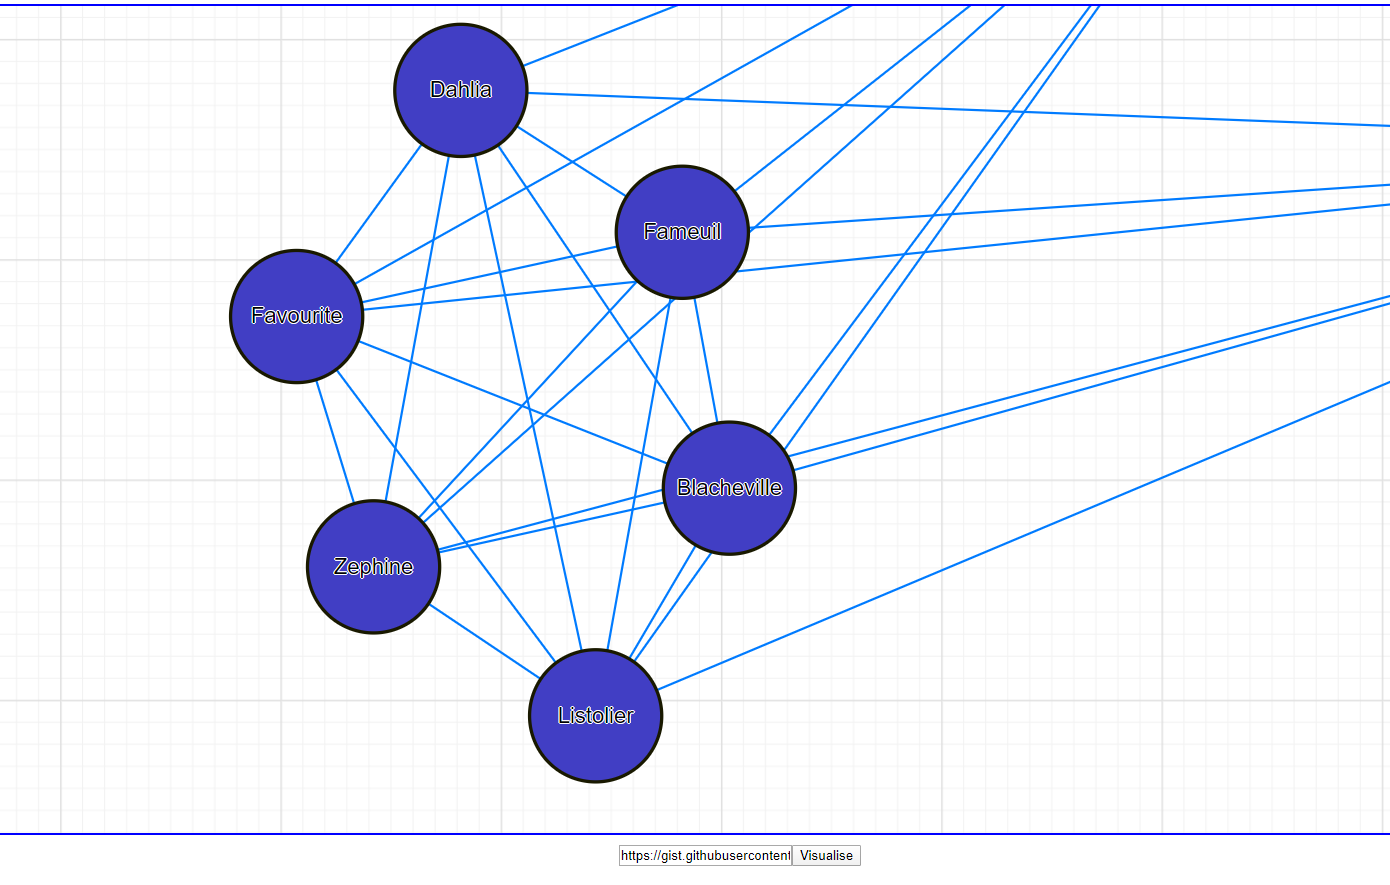
\includegraphics[width=9cm]{rys/zoom.png}}
\label{fig:zoom}
\centering
\end{figure}

\begin{figure}[h]
\caption{Zaznaczenie pojedynczego bytu}
\frame{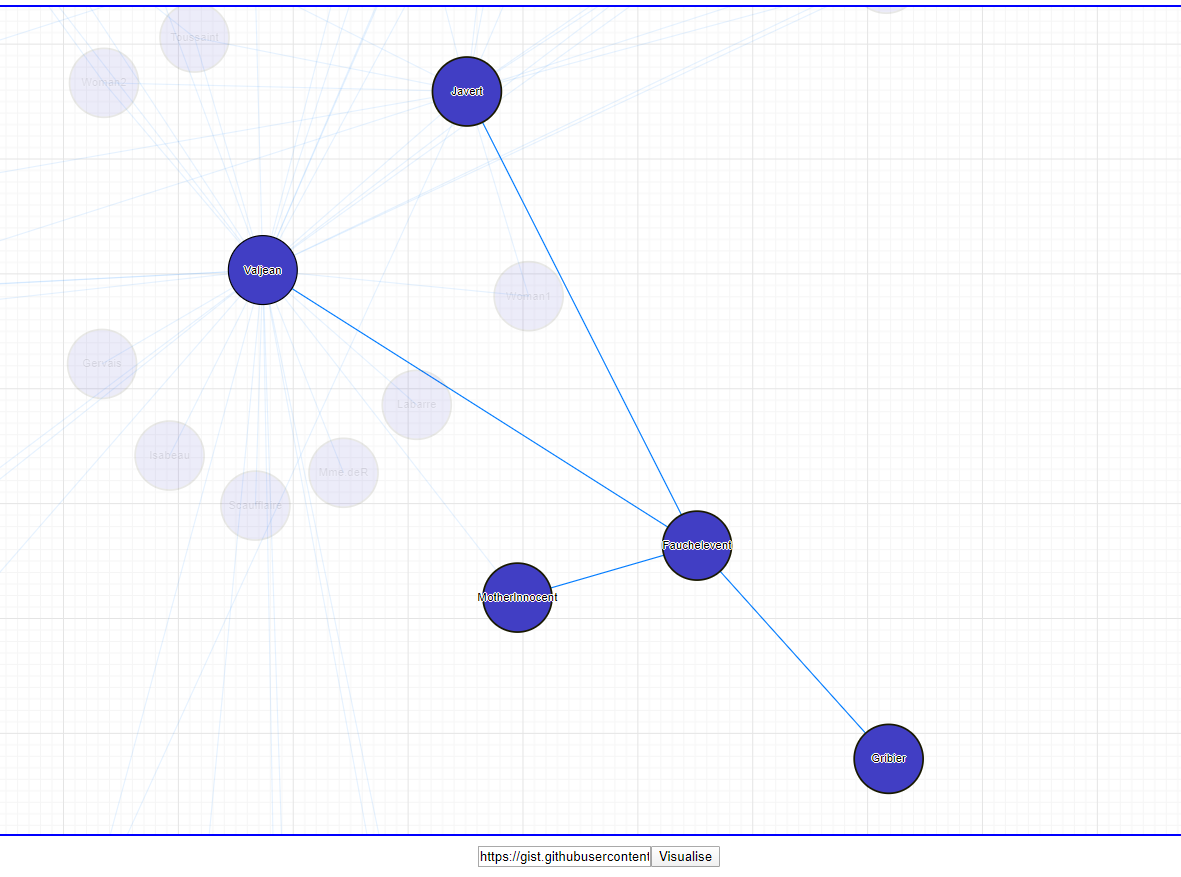
\includegraphics[width=9cm]{rys/highlight.png}}
\label{fig:highlight}
\centering
\end{figure}

Dodatkowo, zaplanowana jest implementacja i przetestowanie użyteczności następujących funkcjonalności:

\begin{itemize}
    \item łączenie bytów mylnie rozróżnionych jako osobne
    \item szczegółowe informacje na temat relacji bytów po najechaniu/kliknięciu myszką na węzeł
    \item zaawansowane opcje generowania grafu. Przykładowo: próg siły relacji bytów od którego łączone są węzły, edycja siły oddziaływającej na węzły
    \item zapis grafu do pamięci użytkownika
\end{itemize}

\newpage

\subsection{Porównanie sposobów generowania obrazu na stronie}
    \subsubsection{SVG "Scalable Vector Graphics"}
        Posiada natywne wsparcie w przeglądarkach internetowych co pozwala osadzić go bezpośrednio w HTML w taki sam sposób, w jaki tworzymy elementy interfejsu użytkownika. Jest łatwy do zrozumienia gdyż składa się z prostych kształtów takich jak prostokąty, koła i linie. Dzięki zintegrowaniu w obiektowym model dokumentu (Document Object Model, DOM) jest prostym sposobem na stworzenie grafiki. Do stworzenia interaktywności, można użyć zdarzeń DOM, które są już wbudowane w przeglądarkę bezpośrednio w węzłach SVG. Do stylizacji węzłów, można wykorzystać CSS.\\
        Główną wadą jest skalowanie liczby węzłów. Ponieważ SVG korzysta z węzłów DOM, które zajmują pamięć, tworzenie SVG z tysiącami węzłów może powodować duży spadek wydajności.\\
        Pomimo problemów ze skalowaniem dla większych woluminów danych, potrafi obsłużyć większość potrzeb wizualizacji. Dzięki łatwości użytkowania i integracji ze standardami HTML jest to najczęściej używana sposób tworzenia grafiki w Internecie.

    \subsubsection{Canvas}
        Html posiada element $<$canvas$>$. Element ten posiada API, które pozwala rysować rasteryzowane obrazy. Ponieważ canvas wymaga rysowania poprzez API potrzebny jest JavaScript aby dynamicznie tworzyć jego zawartość. Dzięki tworzeniu grafiki rastrowej nie jest tak wymagający pamięciowo jak SVG. Możemy dzięki temu szybko narysować tysiące punktów danych w obszarze roboczym. \\
        Wadą tego jest to że efektem renderowania jest obraz. Stworzenie interaktywności wymaga znacznie bardziej złożonych rozwiązań.\\
        Canvas jest wykorzystywany do tworzenia wizualizacji, które renderują więcej punktów danych niż SVG może obsłużyć. Ten zakres jest zwykle w tysiącach punktów danych. Może także obsługiwać animacje danych wydajniej niż SVG. Nadal istnieje górny limit poziomów obsługiwanych danych. Bardziej złożone obliczenia i animacje oraz wizualizacja obszaru roboczego mogą powodować spadek wydajności.
        
    \subsubsection{WebGL}
        Może być wykorzystywany do wizualizacji dużej, złożonej grafiki bez spadku wydajności. WebGL zapewnia API, który umożliwia pisanie kodu niskiego poziomu do tworzenia obrazów rastrowych. Kod jest uruchamiany na GPU komputera zamiast na CPU, umożliwiając równoległe przetwarzanie dużych ilości danych. Dzięki temu grafika 3D oraz duże woluminy informacji oraz animacji mogą być płynnie wykonywane.
        
        
        
    \subsubsection{Podsumowanie}
        W tym projekcie w etapie projektowania uznano że, zastosowanie SVG i D3 jest wystarczające i zostanie ono wykorzystane. W dalszym etapie prac zostanie to przetestowane na danych z przeanalizowanych tekstów i w razie potrzeby zostanie zastosowana biblioteka PIXI.js.
        
\newpage

\subsection{Porównanie bibliotek do wykresów i wizualizacji danych}

   \begin{figure}[h]
        \frame{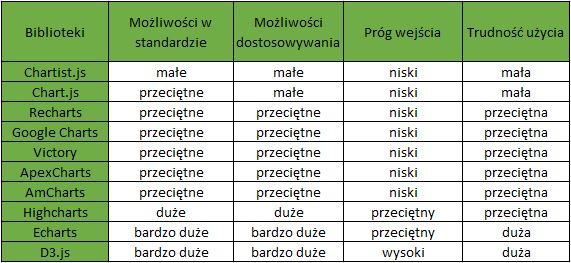
\includegraphics[width=15cm]{rys/porwnanie.JPG}}
        \label{fig:highlight}
        \centering
    \end{figure} 





    \subsubsection{Chartist.js}
        Oferuje wykresy liniowe, punktowe, kołowe, słupkowe i prostą konfigurację. Pozwala na animowanie wykresów, ale nie ma opcji służących interaktywności. Do prezentowania wykresów używa SVG, dlatego nie jest rekomendowana dla dużych kolekcji danych. Wersja zminifikowana to jedyne 10 kB, co nie będzie raczej dużym obciążeniem dla użytkowników strony.

    \subsubsection{Chart.js}
        Jest prostą, ale elastyczną biblioteką do wykresów dla deweloperów i designerów. Prostota wynika między innymi z tego, że do dyspozycji jest 8 typów wykresów, z którymi można jednak wchodzić w interakcję - dzięki standardowym eventom JS.
        Chart.js umożliwia też animowanie wykresów i konfigurację ich podstawowych parametrów. Wykresy są renderowane przy pomocy canvas, a biblioteka w wersji min zajmuje nieco ponad 150kB. Dostępne jest też kilka rozszerzeń, które pozwalają np. na rysowanie nowych wykresów, czy nowe interakcje z wykresami. Największym minusem tej biblioteki jest bardzo ciężkie dopasowanie do własnych, niestandardowych potrzeb; nie da się użyć własnych styli i można modyfikować tylko to, na co pozwala konfiguracja.

        
    \subsubsection{Recharts}
        Jest to biblioteka bazująca na komponentach reactowych i niektórych modułach z D3. Pozwala na rysowanie 9 typów wykresów przy pomocy SVG. W każdym typie można definiować funkcje obsługujące eventy myszki. Przy użyciu Reacta, to może być jeden z najprostszych sposobów na zintegrowanie rysowania wykresów z aplikacją.
        
    \subsubsection{Google Charts}
        Biblioteka od Google oferuje rysowanie interaktywnych wykresów przy pomocy SVG. Zapewnia dostęp do kilkunastu typów wykresów, z którymi można wchodzić w interakcję, w tym przez użycie eventów, ale też kontrolek. Dzięki temu w Google Charts można tworzyć dashboardy, na których prezentowane będą różne, wzajemnie powiązane wykresy. Kolejną ciekawą funkcją jest możliwość połączenia wykresów z danymi z Google Sheets.
        
    \subsubsection{Victory}
        Kolejna biblioteka do produkowania wykresów wyświetlanych jako SVG przy pomocy komponentów reactowych. Victory oferuje 14 typów wykresów oraz możliwość tworzenia własnych, niestandardowych wykresów. Dodatkowo dostępne jest API do animacji, obsługi eventów, motywów oraz ciekawa funkcja przybliżania i wybierania zakresu danych. Victory oferuje też wersję do integracji z React Native.
    
    \subsubsection{ApexCharts}
        ApexCharts to 12 podstawowych typów wykresów oraz możliwość układania ich w dashboardy. Biblioteka pozwala na rysowanie responsywnych, interaktywnych i dynamicznych wykresów, które renderowane są do SVG. Ciekawą funkcją jest dokładanie adnotacji do wykresów, by pomóc użytkownikom zrozumieć dane. Podobnie jak Victory, ApexCharts pozwala na przybliżanie, przewijanie i określanie zakresu wyświetlanych danych. Dodatkowo ta biblioteka jest również dystrybuowana w specjalnej, ułatwiającej integrację wersji dla React i Vue.js.
     
    \subsubsection{AmCharts}
        Biblioteka do rysowania wykresów oraz map napisana w TypeScript. Zapewnia integrację dla aplikacji React, Angular, Vue.js, Ember oraz współpracuje dobrze z Webpackiem, czy RequireJS. Oferuje obecnie 11 typów wizualizacji - w tym chmury słów, lejki, wykresy strunowe i Sankeya. Wszystkie wykresy są generowane w SVG, a biblioteka daje opcje renderowania responsywnego. AmCharts - w przypadku nieodpłatnego używania - wymaga jednak wyświetlenia logo i linku do strony na wszystkich wykresach.

    \subsubsection{Highcharts}
        Biblioteka ta ma już 10 lat i oferuje naprawdę sporo opcji wizualizacji. Znajduje się w niej aż 17 typów wykresów. Pomimo mnogości wykresów i opcji konfiguracyjnych, używanie Highcharts nie jest bardzo skomplikowane. Highcharts jest dostępne za darmo do użytku niekomercyjnego, a rysowanie odbywa się przy pomocy SVG.
    
    \subsubsection{ECharts}
        Biblioteka do wizualizacji danych od Baidu. Twórcy biblioteki skupili się głównie na wizualizacji dużych zbiorów danych. Dlatego znalazło się tu bardzo dużo opcji związanych z interaktywnością - od przełączania zakresów i typów danych, przez tworzenie powiązanych wykresów, rysowanie na powierzchni wykresów, czy wyciąganie danych na zasadzie drag-and-drop. Dodatkowo mamy tu prawie 20 typów wykresów, które można ze sobą kombinować, ponad 600 opcji konfiguracji oraz tryb big data do prezentowania dużych kolekcji. Używa silnika ZRenderer do wyświetlania danych na canvasie. Biblioteka wraz ze wszystkimi wykresami waży około 1MB.
    
    \subsubsection{D3.js}
        D3.js to znacznie więcej niż biblioteka do wizualizacji, a raczej całe podejście do tworzenia dokumentów opartych na danych. Nie jest to monolit, D3 w obecnej wersji jest biblioteką modułową, zawiera w sobie szereg narzędzi wspomagających operacje na danych: takich jak przygotowanie skali, renderowanie wykresów, grafów i map. Biblioteka ta pozwala na dodanie animacji, stylów i customowych zachowań.
        D3.js jest bardzo uniwersalne ale przychodzi to kosztem dużej inwestycji w naukę biblioteki i zrozumienia powiązań wszystkich modułów. Dzięki podejściu D3.js cała biblioteka jest niezwykle lekka, biorąc pod uwagę możliwości. W najnowszej wersji waży niewiele ponad 70kB w wersji min. Wiele innych bibliotek bazuje na D3.js, rozszerzając pewne funkcje, często specjalizując się i ułatwiając konkretne aspekty wizualizacji danych. 
    
    \subsubsection{Pixi.js}
        Jest to biblioteka służąca do renderowania 2D. Pozwala wyrazić deklaratywne drzewo renderowania, podobnie jak SVG. Drzewo renderowania jest jednak przetwarzane tylko w silniku JavaScript, a nie w DOM jak w SVG. W celu przyspieszenia renderowania można wykorzystać tą bibliotekę rysującą wciąż używając D3.js do obliczeń. Biblioteka ta używa domyślnie WebGL ale posiada również wsparcie dla Canvas. 


\begin{figure}[h]
\caption{Przykładowo wygenerowany graf współwystępowania postaci w Les Misérables przy użyciu WebGL oraz biblioteki PIXI.js}
\frame{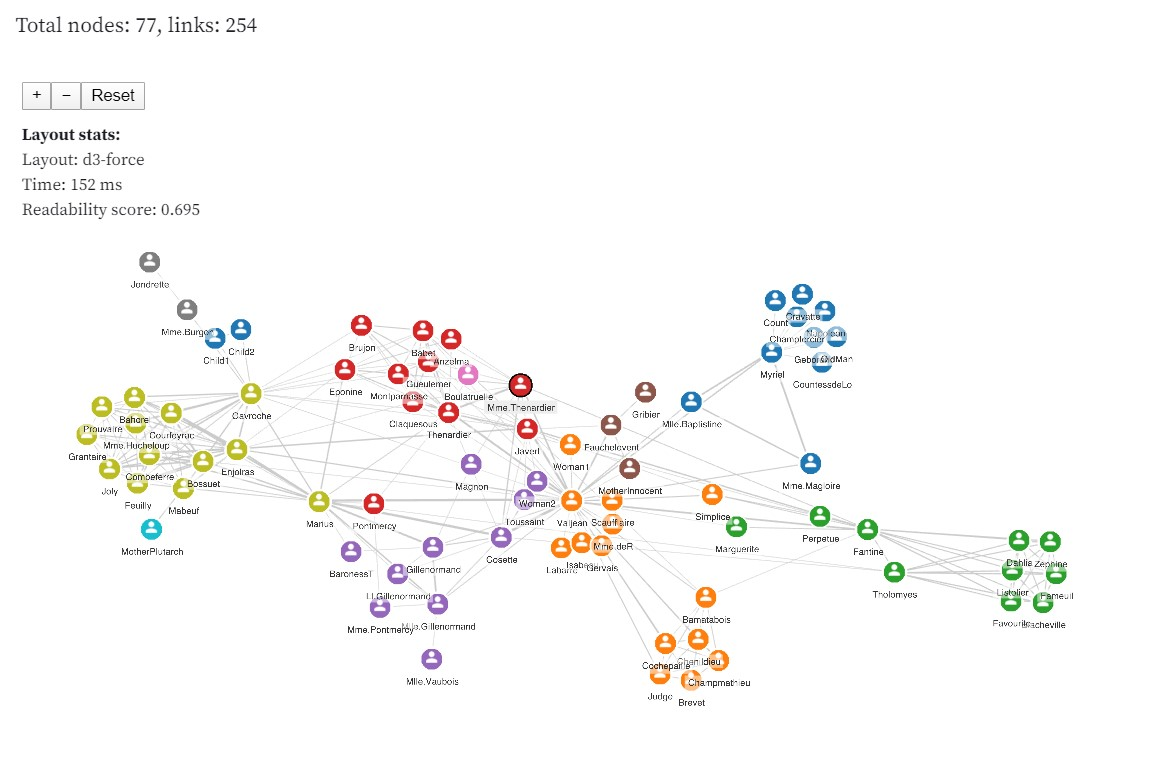
\includegraphics[width=18cm]{rys/webgl+pixi.jpg}}
\label{fig:hotfixToBeChangedLater}%%% THAT LABEL HAS TO BE CHANGED TO BE UNIQUE
\centering
\end{figure}


    \subsubsection{Podsumowanie}
        W aplikacji ze względu na konieczność obsługi dużej ilości danych konieczne jest wykorzystanie biblioteki D3.js. Użycie jej pozwoli na wydajne wygenerowanie grafu bez znacznego spadku wydajności. Pozwoli również konfigurowalną implementacją grafu.



\newpage
\section{Wykorzystane narzędzia zewnętrzne}
\subsection{Clarin-PL}
Clarin-PL to ogólnoeuropejska infrastruktura naukowa, która udostępnia narzędzia do badania dużych zbiorów tekstów. W naszym projekcie wykorzystujemy dwa narzędzia z tej sieci.

\subsubsection{Ner / Liner2}
Jest to narzędzie służące do analizy tekstu oraz rozpoznawania nazw własnych i wyrażeń temporalnych. Narzędzie może być wykorzystywane jako zdalna usługa za pomocą zapytań \texttt{REST} lub jako lokalna instancja (kod dostępny na GitHubie na licencji LGPLv3).

Liner na wejście przyjmuje dowolnie długi tekst, który ma zostać przeanalizowany, a zwraca XML. Wyjściowy \texttt{XML} podzielony jest na fragmenty, zdania i słowa, a do każdego poszczególnego słowa przypisane są informacje o formie podstawowej danego słowa, formie słowa (\texttt{ctag}) oraz dodatkowe adnotacje nt. miejsca lub osoby. W naszym projekcie najbardziej interesują nas adnotacje dotyczące nazw własnych osób.

\subsubsection{Polem}
Polem to narzędzie służące do lematyzacji tekstów języka polskiego. Służy ono do sprowadzania odmienionych wyrazów do ich formy podstawowej (Adamowi -$>$ Adam). Narzędzie to potrafi współpracować z tekstami przetworzonymi za pomocą Linera2, zachowując dodatkowe informacje o danych wyrazach.

Polem, tak jak i Liner, jest dostępny w formie zdalnej usługi, jak i może być uruchomiony lokalnie. Kod Polema również udostępniony jest na licencji LGPLv3.

Narzędzie to przyjmuje na wejście tablicę zawierającą pola zwrócone przez Linera, a zwraca \texttt{JSON}, który zawiera formy podstawowe słów.

\newpage
\section{Metoda szukania powiązania}
% coś o doborze wagno, tutaj obrazki są 
% https://docs.google.com/spreadsheets/d/1PjEAjZ1F2Kp4x7HSWIRXJG0aGkV7MQFsJRegS8vWMEA/edit#gid=0
Opracowano dwa warianty metody polegającej na wydzielaniu z XML-a bytów występujących w poruszającym się po tekście oknie o zmiennej wielkości. Raz wygenerowany z narzędzia \textit{NER} plik XML odpowiadający danemu tekstowi będzie służył do dalszych analiz.

W pierwszej metodzie algorytm rozpoczyna się od zsumowania wystąpień wszystkich bytów w całym wprowadzonym tekście, następnie dokonuje się podziału tekstu na pół. W otrzymanych częściach liczone są wystąpienia bytów. Czynność jest powtarzana aż do osiągnięcia fragmentów tekstu wielkości jednego zdania. Schemat podziału tekstu pokazano na rysunku \ref{fig:polowy}. Wystąpieniom bytów w danym etapie analizy (rozmiar analizowanego fragmentu tekstu) przydzielane są wagi według określonej charakterystyki (stała, liniowa, kwadratowa, etc.) zachowując prawidłowość: im mniejszy analizowany fragment tekstu, tym większa waga.
\begin{figure}[!h]
\caption{Metoda Pierwsza, podział tekstu}
\frame{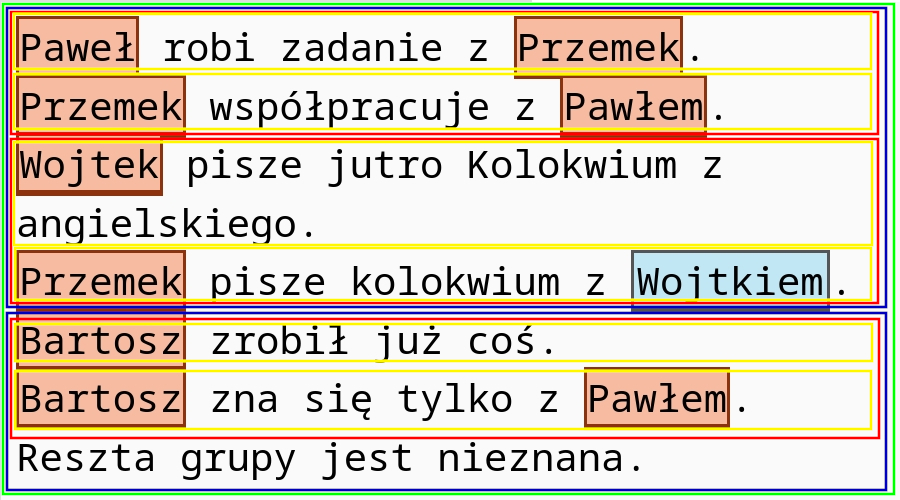
\includegraphics[width=14cm]{rys/polowy.jpg}}
\label{fig:polowy}
\centering
\end{figure}

Druga metoda polega na przemieszczaniu okna po tekście począwszy od pierwszego zdania, aż do końca tekstu w krokach co jedno zdanie, tak jak zaprezentowano na rysunku \ref{fig:plyw}. W każdym kroku, z tekstu znajdującego się w obrębie okna, wydzielane i sumowane będą wystąpienia poszczególnych bohaterów utworu. Każdemu wystąpieniu przydzielana jest waga zależna od rozmiaru okna -- po zakończeniu analizy oknem o największym rozmiarze następuje zmniejszenie okna oraz zwiększenie wagi wystąpienia bytu i powtórzenie analizy z nowym oknem -- większą wagę będą miały dwa byty występujące na obszarze dwóch zdań, niż inne, przeanalizowane na etapie okna o rozmiarze np. 50 zdań. Wystąpienia postaci w obrębie jednego rozmiaru okna, wraz z ilością wystąpień, charakteryzują relację między tymi postaciami. Po osiągnięciu rozmiaru okna równego jednemu zdaniu, relacje pomiędzy bytami z wszystkich etapów są sumowane z uwzględnieniem wag, co daje finalny efekt.
\begin{figure}[!h]
\caption{Metoda Druga, podział tekstu}
\frame{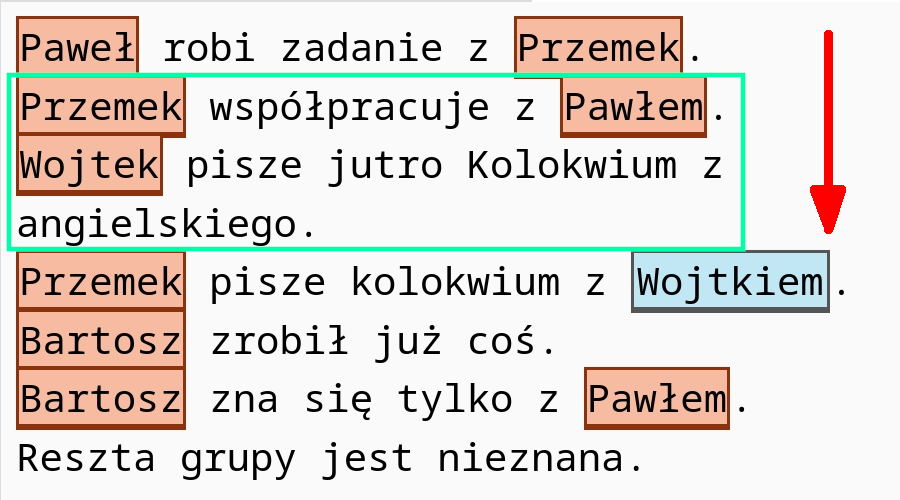
\includegraphics[width=14cm]{rys/plyw.jpg}}
\label{fig:plyw}
\centering
\end{figure}

Powyższe metody zostały przetestowane na prostym tekście:
\begin{quote}
    \textit{
        Paweł robi zadanie z Przemek.
        Przemek współpracuje z Pawłem.
        Wojtek pisze jutro Kolokwium z angielskiego.
        Przemek pisze kolokwium z Wojtkiem.
        Bartosz zrobił już coś.
        Bartosz zna się tylko z Pawłem.
        Reszta grupy jest nieznana.}
\end{quote}

Obie metody były przetestowane dla charakterystyk zmian wag: stałej (równej 1), liniowej, kwadratowej, $n^n$, $n!$. Dodatkowo, w pierwszej metodzie zastosowano dwa różne sposoby na określanie relacji w badanym fragmencie tekstu: poprzez sumowanie wystąpień bytów w danym fragmencie oraz przez wymnażanie.

Poniżej zaprezentowano wyniki analiz przykładowego tekstu metodą pierwszą z wykorzystaniem dodawania i mnożenia oraz metodą drugą.

\begin{figure}[!h]
\caption{Metoda Pierwsza, dodawanie}
\frame{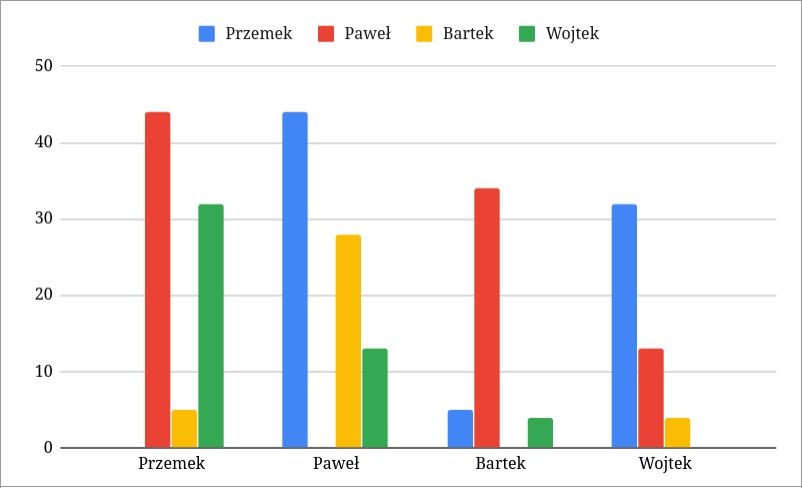
\includegraphics[width=14cm]{rys/met1_add.jpg}}
\label{fig:met1_add}
\centering
\end{figure}

\begin{figure}[!h]
\caption{Metoda Pierwsza, mnożenie}
\frame{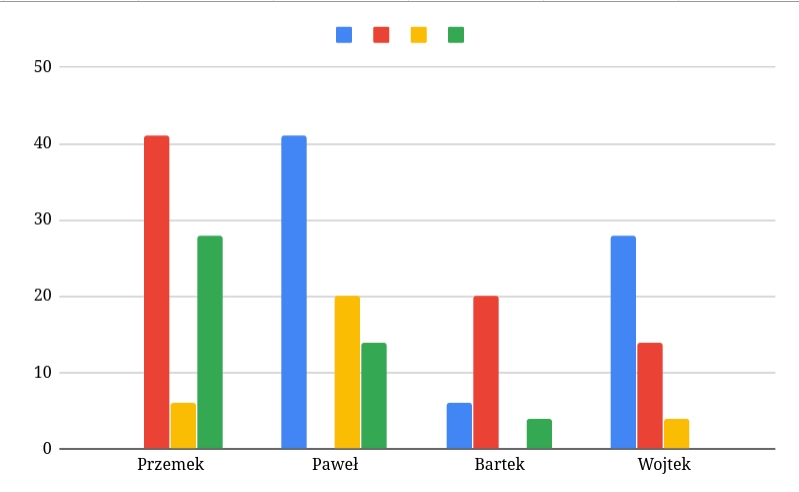
\includegraphics[width=14cm]{rys/met1_mul.jpg}}
\label{fig:met1_mul}
\centering
\end{figure}

\begin{figure}[!h]
\caption{Metoda Druga}
\frame{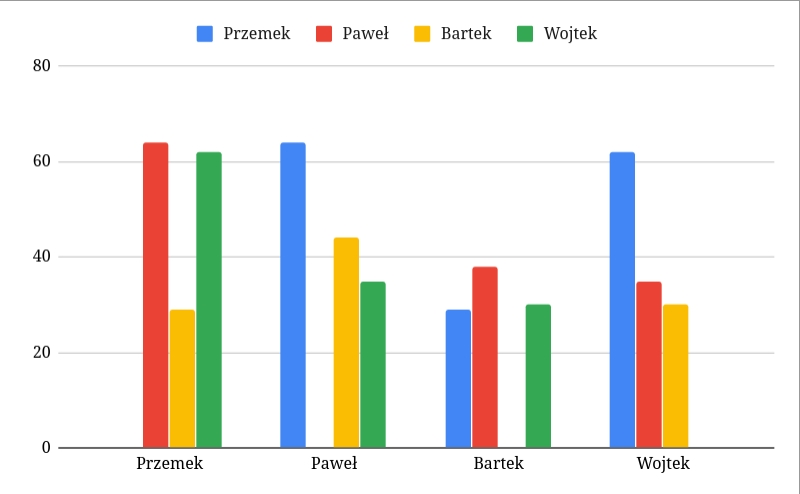
\includegraphics[width=14cm]{rys/met2.jpg}}
\label{fig:met2}
\centering
\end{figure}

\newpage

Parametrem algorytmu jest charakterystyka zwiększania wag. Powyższe wykresy powstały w testach z charakterystyką liniową. Wybór charakterystyki powinien być podyktowany rozmiarem analizowanego tekstu ponieważ algorytm ocenia ilość wystąpień bytów w danym fragmencie. Dla krótkich tekstów różnica między kolejnymi wagami powinna być większa niż w tekstach większych, dlatego druga metoda osiągnęła wyniki bliższe stanowi faktycznemu przy użyciu charakterystyki kwadratowej, co pokazano na rysunku \ref{fig:met2_n^2}.

\begin{figure}[!h]
\caption{Metoda Druga, charakterystyka kwadratowa}
\frame{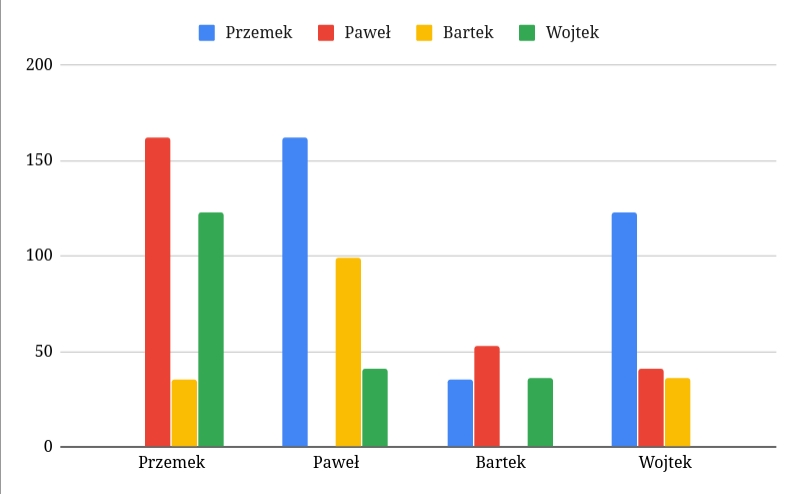
\includegraphics[width=14cm]{rys/met2_n^2.jpg}}
\label{fig:met2_n^2}
\centering
\end{figure}
\newpage
% dobieranie wag - analiza pod względem rozmiaru tekstu
% algo - podział
% 


%\newpage
%\printbibliography

\end{document}

%xDDDDDD